\documentclass{standalone}
\usepackage{tikz}
%\usetikzlibrary{...}
\begin{document}
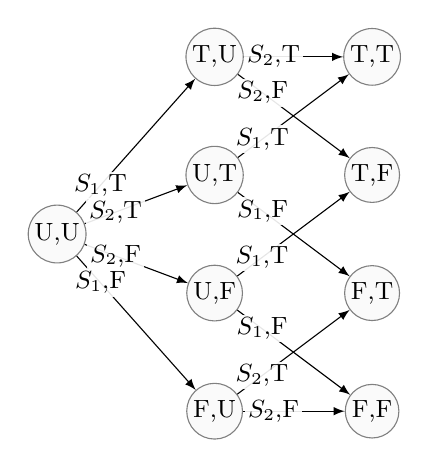
\begin{tikzpicture}[font=\small]

\tikzset{>=latex} % arrow heads

\node[draw=black!50,circle,inner sep=1pt,fill=black!2] (uu) at (0,0) {U,U};

\node[draw=black!50,circle,inner sep=1pt,fill=black!2] (fu) at (2,-2.25) {F,U};
\node[draw=black!50,circle,inner sep=1pt,fill=black!2] (uf) at (2,-0.75) {U,F};
\node[draw=black!50,circle,inner sep=1pt,fill=black!2] (ut) at (2, 0.75) {U,T};
\node[draw=black!50,circle,inner sep=1pt,fill=black!2] (tu) at (2, 2.25) {T,U};


\draw[->] (uu) -- (fu) node[pos=0.20,inner sep=1pt,fill=white,fill opacity=0.9,text opacity=1.0] {$S_1$,F};
\draw[->] (uu) -- (tu) node[pos=0.20,inner sep=1pt,fill=white,fill opacity=0.9,text opacity=1.0] {$S_1$,T};
\draw[->] (uu) -- (uf) node[pos=0.30,inner sep=1pt,fill=white,fill opacity=0.9,text opacity=1.0] {$S_2$,F};
\draw[->] (uu) -- (ut) node[pos=0.30,inner sep=1pt,fill=white,fill opacity=0.9,text opacity=1.0] {$S_2$,T};

\node[draw=black!50,circle,inner sep=1pt,fill=black!2] (ff) at (4,-2.25) {F,F};
\node[draw=black!50,circle,inner sep=1pt,fill=black!2] (ft) at (4,-0.75) {F,T};
\node[draw=black!50,circle,inner sep=1pt,fill=black!2] (tf) at (4, 0.75) {T,F};
\node[draw=black!50,circle,inner sep=1pt,fill=black!2] (tt) at (4, 2.25) {T,T};

\draw[->] (fu) -- (ff) node[pos=0.30,inner sep=1pt,fill=white,fill opacity=0.9,text opacity=1.0] {$S_2$,F};
\draw[->] (fu) -- (ft) node[pos=0.22,inner sep=1pt,fill=white,fill opacity=0.9,text opacity=1.0] {$S_2$,T};

\draw[->] (tu) -- (tf) node[pos=0.22,inner sep=1pt,fill=white,fill opacity=0.9,text opacity=1.0] {$S_2$,F};
\draw[->] (tu) -- (tt) node[pos=0.30,inner sep=1pt,fill=white,fill opacity=0.9,text opacity=1.0] {$S_2$,T};

\draw[->] (uf) -- (ff) node[pos=0.22,inner sep=1pt,fill=white,fill opacity=0.9,text opacity=1.0] {$S_1$,F};
\draw[->] (uf) -- (tf) node[pos=0.22,inner sep=1pt,fill=white,fill opacity=0.9,text opacity=1.0] {$S_1$,T};

\draw[->] (ut) -- (ft) node[pos=0.22,inner sep=1pt,fill=white,fill opacity=0.9,text opacity=1.0] {$S_1$,F};
\draw[->] (ut) -- (tt) node[pos=0.22,inner sep=1pt,fill=white,fill opacity=0.9,text opacity=1.0] {$S_1$,T};

\end{tikzpicture}%
\end{document}
